\documentclass[a4paper,12pt]{article}
\usepackage[utf8]{inputenc}
\usepackage[T1]{fontenc}
\usepackage[french]{babel}
\usepackage{amsmath, amssymb, amsfonts}
\usepackage{graphicx}
\usepackage{hyperref}
\usepackage{geometry}
\usepackage{enumitem}
\usepackage{titlesec}
\usepackage{setspace}
\usepackage{tikz}
\usepackage{pgfplots}
\usepackage[most]{tcolorbox}
\newtcolorbox{propsBox}[1][]{
  colback=red!5!white,
  colframe=red!75!black,
  title={\textbf{Propriétés :} #1},
}

% --- Langue et encodage ---
\usepackage[utf8]{inputenc}     % Encodage UTF-8 (caractères accentués)
\usepackage[T1]{fontenc}        % Bon rendu typographique des caractères accentués
\usepackage[french]{babel}      % Traduction des éléments LaTeX en français

% --- Mathématiques ---
\usepackage{amsmath, amssymb, amsfonts}

% --- Graphiques et diagrammes ---
\usepackage{tikz}               % Pour les dessins vectoriels
\usetikzlibrary{arrows.meta, positioning, shapes, calc} 
% ↑ Librairies TikZ utilisées :
%   - arrows.meta : pour les flèches modernes (>=latex)
%   - positioning : pour placer facilement les nœuds (ex: right=2cm of A)
%   - shapes : pour les rectangles arrondis, cercles, etc.
%   - calc : pour faire des positions relatives précises

\usepackage{pgfplots}           % Pour tracer les courbes (sigmoid, tanh, etc.)
\pgfplotsset{compat=1.18}

% --- Mise en page générale ---
\usepackage{geometry}
\geometry{margin=2.5cm}

\usepackage{setspace}
\setstretch{1.2}                % Interligne légèrement augmenté

\usepackage{enumitem}           % Meilleur contrôle des listes (itemize/enumerate)

\usepackage{hyperref}           % Liens cliquables dans la table des matières

\usepackage[ruled,vlined,linesnumbered]{algorithm2e}

\pgfplotsset{compat=1.18}
% \documentclass[tikz,border=3.14mm]{standalone}
\geometry{margin=2.5cm}
\setstretch{1.2}



\titleformat{\section}{\normalfont\Large\bfseries}{\thesection.}{0.5em}{}
\titleformat{\subsection}{\normalfont\large\bfseries}{\thesubsection.}{0.5em}{}

\title{Principe et Implémentation d'un Réseau de Neurones Artificiel}
\author{Mohamed Ahmed Mohamed Lemine}
\date{\today}

\begin{document}

\maketitle

\begin{abstract}
Les réseaux de neurones artificiels (ANN) constituent la base du \textit{Deep Learning}. Ce document présente les principes fondamentaux d’un neurone artificiel, la modélisation mathématique d’un réseau multicouche (MLP), les principales fonctions de coût, ainsi que les méthodes d’optimisation comme la descente de gradient et ses variantes. L’algorithme de rétropropagation est ensuite détaillé avant de présenter une implémentation en Python et une application sur le dataset MNIST pour la reconnaissance de chiffres manuscrits.
\end{abstract}

\tableofcontents
\newpage

% =========================
\section{Introduction}

\subsection{Définition d'un neurone}
Un neurone artificiel est une unité de calcul inspirée du neurone biologique. Il prend des entrées $x_1, x_2, \dots, x_n$, les pondère par des coefficients $w_i$, ajoute un biais $b$, et applique une fonction d’activation $f$ :
\[
y = f\left(\sum_{i=1}^{n} w_i x_i + b \right)
\]
L’objectif est d’apprendre les poids $w_i$ et le biais $b$ pour minimiser l’erreur entre la sortie prédite et la valeur réelle.

\bigskip

\noindent Voici une représentation schématique d’un neurone artificiel :



\begin{center}
    
\begin{tikzpicture}[
    neuron/.style={circle, draw=black, thick, minimum size=1.5cm},
    input/.style={circle, draw=black, thick, minimum size=0.8cm},
    >=stealth,
    font=\small
]

% Neurone
\node[neuron] (neuron) at (4,0) {$\Sigma \mid$ $f$};

% Entrées
\node[input] (x1) at (0,2) {$x_1$};
\node[input] (x2) at (0,1) {$x_2$};
\node (dots) at (0,0) {$\vdots$};
\node[input] (xn) at (0,-1) {$x_n$};

% Biais
\node[input] (bias) at (4,-2) {$b$};

% Sortie
\node (y) at (7,0) {$y = f\left(\sum\limits_{i=1}^{n} w_i x_i + b\right)$};

% Connexions entrées → neurone
\draw[->] (x1) -- node[above, pos=0.7] {$w_1$} (neuron);
\draw[->] (x2) -- node[above, pos=0.7] {$w_2$} (neuron);
\draw[->] (xn) -- node[above, pos=0.7] {$w_n$} (neuron);

% Connexion biais → neurone
\draw[->] (bias) -- node[below right=1pt, pos=0.9] {$1$} (neuron);

% Connexion neurone → sortie
\draw[->] (neuron) -- (y);

% Ligne pointillée pour les connexions manquantes
\draw[dashed] (x2) -- (dots);
\draw[dashed] (dots) -- (xn);

\end{tikzpicture}
\end{center}


\bigskip


\subsection{Les fonctions d'activation}

\subsubsection*{Définition}
Une \textbf{fonction d’activation} introduit de la \textit{non-linéarité} dans un réseau de neurones.  
Sans cette non-linéarité, un réseau multicouche se comporterait comme une simple régression linéaire, incapable de modéliser des relations complexes.  

Ainsi, chaque neurone applique une fonction $f$ sur la combinaison linéaire de ses entrées :
\[
y = f\left(\sum_{i=1}^{n} w_i x_i + b\right)
\]
Les principales fonctions d’activation utilisées dans la pratique sont : la sigmoïde, la tangente hyperbolique, ReLU et softmax.

\bigskip

% ------------------------------
\subsubsection*{a. Sigmoïde}
La fonction sigmoïde transforme toute valeur réelle en une valeur comprise entre 0 et 1 :
\[
f(x) = \frac{1}{1 + e^{-x}}
\]
\textbf{Dérivée :}
\[
f'(x) = \frac{e^{-x}}{\left( 1+ e^{-x} \right)^2} = f(x)(1 - f(x))
\]

\textbf{Propriétés :}
\begin{itemize}[label=$\bullet$]
    \item Bornée : $f(x) \in ]0,1[$
    \item Lisse et monotone croissante
    \item Bonne interprétation probabiliste
    \item \textit{Inconvénient} : saturations pour $|x|$ grands $\Rightarrow$ gradients proches de 0 (vanishing gradient)
\end{itemize}


\begin{center}
\begin{tikzpicture}
    \begin{axis}[
        width=8cm, height=5cm,
        xlabel={$x$}, ylabel={$f(x)$},
        axis lines=middle,
        samples=200,
        domain=-8:8,
        ymin=-0.1, ymax=1.1,
        grid=major,
        title={Sigmoïde}
    ]
    \addplot[blue, thick] {1/(1 + exp(-x))};
    \end{axis}
\end{tikzpicture}
\end{center}



\bigskip

% ------------------------------
\subsubsection*{b. Tangente hyperbolique (Tanh)}
La fonction Tanh est une version centrée de la sigmoïde :
\[
f(x) = \tanh(x) = \frac{e^{x} - e^{-x}}{e^{x} + e^{-x}}
\]
\textbf{Dérivée :}
\[
f'(x) = 1 - f(x)^2
\]

\textbf{Propriétés :}
\begin{itemize}[label=$\bullet$]
    \item Bornée : $f(x) \in ]-1,1[$
    \item Zéro-centre la sortie (accélère l’apprentissage)
    \item \textit{Inconvénient} : toujours sujette au problème de gradient qui disparaît pour $|x|$ grand
\end{itemize}


\begin{center}
\begin{tikzpicture}
    \begin{axis}[
        width=8cm, height=5cm,
        xlabel={$x$}, ylabel={$f(x)$},
        axis lines=middle,
        samples=200,
        domain=-5:5,
        ymin=-1.2, ymax=1.2,
        grid=major,
        title={Tangente hyperbolique}
    ]
    \addplot[red, thick] {tanh(x)};
    \end{axis}
\end{tikzpicture}
\end{center}

\bigskip


\subsubsection*{c. ReLU (Rectified Linear Unit)}

La fonction ReLU est définie comme :
\[
f(x) = \max(0, x)
\]
\textbf{Dérivée :}
\[
f'(x) =
\begin{cases}
1 & \text{si } x > 0,\\
0 & \text{sinon.}
\end{cases}
\]

\textbf{Propriétés :}
\begin{itemize}[label=$\bullet$]
    \item Simple et très efficace pour les réseaux profonds
    \item Pas de saturation pour les valeurs positives
    \item \textit{Inconvénient} : les neurones peuvent “mourir” si $x < 0$ trop souvent (\textit{dying ReLU})
\end{itemize}


\begin{center}
\begin{tikzpicture}
    \begin{axis}[
        width=8cm, height=5cm,
        xlabel={$x$}, ylabel={$f(x)$},
        axis lines=middle,
        samples=200,
        domain=-5:5,
        ymin=-1, ymax=6,
        grid=major,
        title={ReLU}
    ]
    \addplot[thick, color=purple] {max(0,x)};
    \end{axis}
\end{tikzpicture}
\end{center}


\bigskip
% \subsubsection*{d. Softmax}



% \bigskip

\noindent
\textbf{Résumé :}  
\begin{center}
\begin{tabular}{|c|c|c|c|}
\hline
\textbf{Fonction} & \textbf{Forme} & \textbf{Plage} & \textbf{Dérivée principale} \\
\hline
Sigmoïde & $\frac{1}{1 + e^{-x}}$ & (0,1) & $f(1-f)$ \\
\hline
Tanh & $\tanh(x)$ & (-1,1) & $1-f^2$ \\
\hline
ReLU & $\max(0,x)$ & [0,$\infty$) & $1_{x>0}$ \\
\hline
% Softmax & $\frac{e^{x_i}}{\sum_j e^{x_j}}$ & [0,1] & $f_i(1-f_i)$ ou $-f_if_j$ \\
% \hline
\end{tabular}
\end{center}




\subsection{Généralisation : le Perceptron Multicouche (MLP)}

% Un perceptron multicouche (MLP) est une composition de plusieurs neurones organisés en couches :
% \[
% \hat{y} = f^{(L)}(W^{(L)} f^{(L-1)}(W^{(L-1)} \dots f^{(1)}(W^{(1)}x + b^{(1)}) + \dots + b^{(L-1)}) + b^{(L)})
% \]
% Les couches cachées permettent au modèle d’apprendre des représentations complexes des données.



\subsubsection*{Définition}

Un \textbf{Perceptron Multicouche} (ou \textit{Multi-Layer Perceptron}, MLP) est une extension naturelle du neurone artificiel à plusieurs couches.  
Il est constitué :
\begin{itemize}[label=$\bullet$]
    \item d’une \textbf{couche d’entrée}, qui reçoit le vecteur des caractéristiques $x \in \mathbb{R}^{n_0}$,
    \item d’une ou plusieurs \textbf{couches cachées}, chacune composée de plusieurs neurones,
    \item d’une \textbf{couche de sortie}, qui produit la prédiction finale $\hat{y}$.
\end{itemize}

Chaque couche effectue une transformation \textbf{affine} suivie d’une \textbf{fonction d’activation non linéaire}.  
Ainsi, la sortie d’une couche devient l’entrée de la couche suivante.

\begin{center}
\begin{tikzpicture}[>=latex, scale=1, every node/.style={transform shape}]
    % Layer 0 (Input)
    \node[circle, draw, minimum size=0.7cm] (I1) at (0,1.5) {};
    \node[circle, draw, minimum size=0.7cm] (I2) at (0,0) {};
    \node[circle, draw, minimum size=0.7cm] (I3) at (0,-1.5) {};

    % Hidden layer 1
    \node[circle, draw, fill=gray!10, minimum size=0.7cm] (H1) at (3,2) {};
    \node[circle, draw, fill=gray!10, minimum size=0.7cm] (H2) at (3,0.5) {};
    \node[circle, draw, fill=gray!10, minimum size=0.7cm] (H3) at (3,-1) {};
    \node[circle, draw, fill=gray!10, minimum size=0.7cm] (H4) at (3,-2.5) {};

    % Hidden layer 2
    \node[circle, draw, fill=gray!10, minimum size=0.7cm] (Htwo1) at (6,1.5) {};
    \node[circle, draw, fill=gray!10, minimum size=0.7cm] (Htwo2) at (6,0) {};
    \node[circle, draw, fill=gray!10, minimum size=0.7cm] (Htwo3) at (6,-1.5) {};

    % Output layer
    \node[circle, draw, fill=gray!20, minimum size=0.7cm] (O) at (9,0) {};

    % Connections Input -> Hidden1
    \foreach \i in {1,2,3}
        \foreach \j in {1,2,3,4}
            \draw[->, thin] (I\i) -- (H\j);

    % Connections Hidden1 -> Hidden2
    \foreach \i in {1,2,3,4}
        \foreach \j in {1,2,3}
            \draw[->, thin] (H\i) -- (Htwo\j);

    % Connections Hidden2 -> Output
    \foreach \i in {1,2,3}
        \draw[->, thin] (Htwo\i) -- (O);

    % Labels
    \node at (0,-3.3) {Entrée $x$};
    \node at (3,-3.3) {Couches cachées};
    \node at (9,-3.3) {Sortie $\hat{y}$};
\end{tikzpicture}
\end{center}


\subsubsection*{Notations}

On note :
\begin{itemize}[label=$\bullet$]
    \item $L$ : le nombre total de couches (hors entrée),
    \item $n_l$ : le nombre de neurones dans la couche $l$,
    \item $W^{(l)} \in \mathbb{R}^{n_l \times n_{l-1}}$ : la matrice des poids reliant la couche $(l-1)$ à la couche $l$,
    \item $b^{(l)} \in \mathbb{R}^{n_l}$ : le vecteur des biais de la couche $l$,
    \item $a^{(l)} \in \mathbb{R}^{n_l}$ : le vecteur des activations (sorties) de la couche $l$.
\end{itemize}

\noindent
Ainsi, pour la couche $l$ :
\[
z^{(l)} = W^{(l)} a^{(l-1)} + b^{(l)}, \qquad a^{(l)} = f^{(l)}(z^{(l)}),
\]
où $f^{(l)}$ est la fonction d’activation choisie pour la couche $l$.


\subsubsection*{Formulation générale du MLP}

La propagation avant (\textit{forward propagation}) d'un réseau MLP s'écrit de manière récursive :
\[
\begin{cases}
a^{(0)} = x, & \text{(entrée)} \\
a^{(l)} = f^{(l)}(W^{(l)} a^{(l-1)} + b^{(l)}), & \forall l = 1, 2, \dots, L-1 \\
\hat{y} = f^{(L)}(W^{(L)} a^{(L-1)} + b^{(L)}), & \text{(sortie finale)}
\end{cases}
\]

\noindent
où :
\begin{itemize}[label=$\bullet$]
    \item $f^{(l)}$ peut varier selon les couches 
    \item $\hat{y}$ est la prédiction du réseau,
    \item le vecteur $x$ est l’entrée du modèle.
\end{itemize}

\bigskip
\noindent
On peut résumer la transformation complète du réseau comme une \textbf{composition de fonctions de couche}.  
Pour chaque couche $l$, on définit :
\[
g^{(l)}(x) := f^{(l)}\big(W^{(l)} x + b^{(l)}\big)
\]
où $g^{(l)} : \mathbb{R}^{n_{l-1}} \to \mathbb{R}^{n_l}$ représente la transformation complète réalisée par la couche $l$.

Ainsi, la sortie finale du réseau (\textit{forward pass}) s’écrit comme une composition de ces transformations :
\[
\hat{y} = g^{(L)} \circ g^{(L-1)} \circ \dots \circ g^{(1)}(x)
\]

\vspace{2cm}

\subsubsection*{Remarques}
\begin{itemize}[label=$\bullet$]
    \item Le MLP est un \textbf{approximateur universel} : avec suffisamment de neurones et de couches, il peut approximer n'importe quelle fonction continue.
    \item Le nombre de couches et de neurones influence la capacité du modèle et sa tendance au surapprentissage.
    \item Les fonctions d’activation assurent la non-linéarité nécessaire pour modéliser des relations complexes.
\end{itemize}


% ===================
\newpage

\section{Fonction de coût}

\subsection*{Introduction}

L'objectif de l'apprentissage supervisé est d'ajuster les paramètres du modèle (poids et biais) afin de minimiser l'erreur entre les prédictions du réseau $\hat{y}$ et les vraies valeurs $y$.  
Pour quantifier cette erreur, on introduit une \textbf{fonction de coût} (ou \textit{loss function}) notée $L(y, \hat{y})$.

\medskip

Une bonne fonction de coût doit :
\begin{itemize}[label=$\bullet$]
    \item être différentiable (pour permettre l’optimisation par descente de gradient),
    \item croître lorsque les prédictions s’éloignent de la vérité,
    \item refléter correctement la nature du problème (classification, régression, etc.).
\end{itemize}

Les fonctions de coût les plus utilisées sont :
\begin{itemize}[label=$\circ$]
    \item \textbf{MSE (Mean Squared Error)} pour les tâches de régression ;
    \item \textbf{Cross-Entropy} pour les tâches de classification.
\end{itemize}



\subsection{Erreur quadratique moyenne (MSE)}

\subsubsection*{Définition}

L’erreur quadratique moyenne (MSE) mesure la moyenne des carrés des écarts entre les valeurs réelles et prédites :
\[
L_{MSE}(y, \hat{y}) = \frac{1}{N} \sum_{i=1}^{N} (y_i - \hat{y}_i)^2
\]
où :
\begin{itemize}[label=$\bullet$]
    \item $y_i$ : la valeur réelle de la $i$\textsuperscript{ème} observation,
    \item $\hat{y}_i$ : la valeur prédite correspondante,
    \item $N$ : le nombre total d’échantillons.
\end{itemize}

\noindent
La MSE pénalise fortement les grandes erreurs, car celles-ci sont élevées au carré.


\subsubsection*{Définition dans le contexte des réseaux de neurones}

Dans un réseau de neurones, la MSE évalue la différence entre les sorties du réseau $\hat{y}^{(i)} = \mathcal{F}(x^{(i)}; \Theta)$ et les vraies cibles $y^{(i)}$ pour l’ensemble des échantillons du jeu d’entraînement :
\[
L_{MSE}(\Theta) = \frac{1}{N} \sum_{i=1}^{N} \left\| y^{(i)} - \mathcal{F}(x^{(i)}; \Theta) \right\|_2^2
\]
où :
\begin{itemize}[label=$\bullet$]
    \item $\mathcal{F}(x^{(i)}; \Theta)$ désigne la sortie du réseau pour l’entrée $x^{(i)}$ avec paramètres $\Theta = \{W^{(l)}, b^{(l)}\}_{l=1}^L$,
    \item $y^{(i)}$ est le vecteur de sortie attendu (valeur réelle),
    \item $\|\cdot\|_2$ représente la norme euclidienne.
\end{itemize}

\noindent
Cette formulation montre que la fonction de coût dépend implicitement des poids et biais du réseau à travers $\mathcal{F}(x^{(i)}; \Theta)$.  
Minimiser $L_{MSE}(\Theta)$ revient donc à ajuster les paramètres $\Theta$ afin que le réseau reproduise au mieux les valeurs cibles.


\bigskip

\begin{center}
\begin{tikzpicture}[>=latex, thick, scale=1, every node/.style={transform shape}]

% === Bloc 1 : Données d'entrée ===
\node[draw, rounded corners, fill=blue!10, minimum width=5cm, minimum height=2.3cm, align=center] (data) 
{\textbf{Données d'entraînement} \\[0.3em]
$(x_1, y_1)$ \\[-0.2em]
$\vdots$ \\[-0.2em]
$(x_N, y_N)$};


\node[draw, rounded corners, fill=orange!10, minimum width=6cm, minimum height=5cm, align=center, below=1.5cm of data] (nn)
{\textbf{Réseau de Neurones}\\[0.4em]
\begin{tikzpicture}[scale=0.7, every node/.style={transform shape}]
    % --- Premier mini-réseau ---
    % Entrée et sortie
    \node[circle, draw, fill=gray!10, minimum size=0.5cm] (i1) at (0,1.5) {};
    \node[circle, draw, fill=gray!10, minimum size=0.5cm] (h11) at (1,1.9) {};
    \node[circle, draw, fill=gray!10, minimum size=0.5cm] (h12) at (1,1.1) {};
    \node[circle, draw, fill=gray!10, minimum size=0.5cm] (o1) at (2,1.5) {};
    % Connexions
    \draw[->] (i1) -- (h11);
    \draw[->] (i1) -- (h12);
    \draw[->] (h11) -- (o1);
    \draw[->] (h12) -- (o1);
    % Labels et flèches d'entrée/sortie
    \node[left=0.5cm of i1] (x1) {$x_1$};
    \draw[->] (x1) -- (i1);
    \node[right=0.5cm of o1] (y1) {$\hat{y}_1$};
    \draw[->] (o1) -- (y1);

    % --- Points de suspension ---
    \node at (1,2.5) {$\vdots$};

    % --- Dernier mini-réseau ---
    \node[circle, draw, fill=gray!10, minimum size=0.5cm] (in) at (0,-1.3) {};
    \node[circle, draw, fill=gray!10, minimum size=0.5cm] (hn1) at (1,-0.9) {};
    \node[circle, draw, fill=gray!10, minimum size=0.5cm] (hn2) at (1,-1.7) {};
    \node[circle, draw, fill=gray!10, minimum size=0.5cm] (on) at (2,-1.3) {};
    % Connexions
    \draw[->] (in) -- (hn1);
    \draw[->] (in) -- (hn2);
    \draw[->] (hn1) -- (on);
    \draw[->] (hn2) -- (on);
    % Labels et flèches
    \node[left=0.5cm of in] (xN) {$x_N$};
    \draw[->] (xN) -- (in);
    \node[right=0.5cm of on] (yN) {$\hat{y}_N$};
    \draw[->] (on) -- (yN);

\end{tikzpicture}
};

% === Flèche vers le réseau ===
\draw[->, thick] (data.south) -- node[right]{\scriptsize Entrée des $x_i$ dans le réseau} (nn.north);

% === Bloc 3 : Sorties ===
\node[draw, rounded corners, fill=green!10, minimum width=5cm, minimum height=2.2cm, align=center, below=1.8cm of nn] (out)
{\textbf{Sorties agrégées} \\[0.4em]
$\hat{y} = (\hat{y}_1, \dots, \hat{y}_N)$ \\[0.2em]
$y = (y_1, \dots, y_N)$};

\draw[->, thick] (nn.south) -- node[right]{\scriptsize Prédictions du réseau} (out.north);

% === Bloc 4 : Fonction de coût ===
\node[draw, rounded corners, fill=red!10, minimum width=5.5cm, minimum height=1.7cm, align=center, below=1.5cm of out] (loss)
{\textbf{Fonction de coût MSE} \\[0.4em]
$L_{MSE} = \frac{1}{N} \sum_{i=1}^{N} (y_i - \hat{y}_i)^2$};

\draw[->, thick] (out.south) -- node[right]{\scriptsize Calcul de l'erreur globale} (loss.north);

\end{tikzpicture}
\end{center}






% =========================

% \section{Descente de gradient}

% \subsection{Introduction}
% La descente de gradient consiste à ajuster les paramètres du réseau pour minimiser la fonction de coût :
% \[
% w_{ij} \leftarrow w_{ij} - \eta \frac{\partial L}{\partial w_{ij}}
% \]
% où $\eta$ est le taux d’apprentissage.

% \subsection{Batch Gradient Descent}
% L’ensemble complet des données est utilisé pour calculer le gradient à chaque mise à jour. C’est précis mais lent.

% \subsection{Mini-Batch Gradient Descent}
% Les données sont divisées en petits lots (\textit{mini-batches}), combinant rapidité et stabilité :
% \[
% \text{mise à jour après chaque mini-lot de taille } m
% \]

% \subsection{Stochastic Gradient Descent (SGD)}
% Chaque exemple est utilisé pour une mise à jour :
% \[
% w_{ij} \leftarrow w_{ij} - \eta \frac{\partial L(x_i)}{\partial w_{ij}}
% \]

% \subsection{Adam Optimizer}
% L’algorithme Adam combine l’adaptation du taux d’apprentissage et le momentum :
% \[
% m_t = \beta_1 m_{t-1} + (1 - \beta_1) g_t, \quad v_t = \beta_2 v_{t-1} + (1 - \beta_2) g_t^2
% \]
% \[
% \theta_t = \theta_{t-1} - \eta \frac{m_t / (1 - \beta_1^t)}{\sqrt{v_t / (1 - \beta_2^t)} + \epsilon}
% \]

% % =========================





\section{Algorithme de Backpropagation}



\subsection{Définition}

L'\textbf{algorithme de rétropropagation du gradient} (ou \textit{Backpropagation}) est une méthode permettant de calculer efficacement les gradients de la fonction de coût par rapport aux paramètres du réseau de neurones (poids et biais).  

\medskip
Il s'agit du cœur de l'apprentissage des réseaux de neurones, car il permet la mise à jour des paramètres via une méthode d’optimisation (comme la descente de gradient).  

\begin{itemize}[label=$\bullet$]
    \item Il repose sur l’application répétée de la \textbf{règle de la chaîne} pour propager l’erreur depuis la couche de sortie jusqu’aux couches d’entrée.
    \item L’objectif est de minimiser la fonction de perte $L(\Theta)$ en ajustant les paramètres $\Theta = \{W^{(l)}, b^{(l)}\}_{l=1}^L$.
\end{itemize}


\subsection*{Notations générales}

Soit un réseau de neurones comportant $L$ couches (hors couche d’entrée).  
Pour chaque couche $l \in \{1, 2, \dots, L\}$, on définit les éléments suivants :

\begin{itemize}[label=$\bullet$]
    \item $n_l$ : nombre de neurones dans la couche $l$.
    \item $W^{(l)} \in \mathbb{R}^{n_l \times n_{l-1}}$ : matrice des poids reliant la couche $(l-1)$ à la couche $l$ :
    \[
    W^{(l)} =
    \begin{bmatrix}
    w^{(l)}_{1,1} & w^{(l)}_{1,2} & \cdots & w^{(l)}_{1,n_{l-1}} \\
    w^{(l)}_{2,1} & w^{(l)}_{2,2} & \cdots & w^{(l)}_{2,n_{l-1}} \\
    \vdots & \vdots & \ddots & \vdots \\
    w^{(l)}_{n_l,1} & w^{(l)}_{n_l,2} & \cdots & w^{(l)}_{n_l,n_{l-1}}
    \end{bmatrix}
    \]
    où $w^{(l)}_{i,j}$ représente le poids reliant la sortie du neurone $j$ de la couche $(l-1)$ à l’entrée du neurone $i$ de la couche $l$.

    \item $b^{(l)} \in \mathbb{R}^{n_l}$ : vecteur des biais de la couche $l$ :
    \[
    b^{(l)} =
    \begin{bmatrix}
    b^{(l)}_1 \\ b^{(l)}_2 \\ \vdots \\ b^{(l)}_{n_l}
    \end{bmatrix}
    \]

    \item $f^{(l)} : \mathbb{R}^{n_l} \to \mathbb{R}^{n_l}$ : fonction d’activation appliquée élément par élément :
    \[
    f^{(l)}(z) =
    \begin{bmatrix}
    f^{(l)}(z_1) \\
    f^{(l)}(z_2) \\
    \vdots \\
    f^{(l)}(z_{n_l})
    \end{bmatrix}
    \]

    \item $a^{(l)} \in \mathbb{R}^{n_l}$ : vecteur des activations (sorties) de la couche $l$.
    \item $z^{(l)} \in \mathbb{R}^{n_l}$ : vecteur des combinaisons linéaires avant activation :
    \[
    z^{(l)} = W^{(l)} a^{(l-1)} + b^{(l)} \quad \text{et} \quad a^{(l)} = f^{(l)}(z^{(l)}).
    \]
\end{itemize}


\subsection*{Objectif}

Soit $L(\Theta)$ la \textbf{fonction de perte globale} du réseau, qui dépend de tous les paramètres $\Theta = \{W^{(l)}, b^{(l)}\}_{l=1}^L$ :
\[
L(\Theta) = \frac{1}{N} \sum_{i=1}^N \ell\big(y^{(i)}, \hat{y}^{(i)}(\Theta)\big)
\]
où $\ell$ est la perte pour un échantillon donné (par exemple MSE ou Cross-Entropy), et $\hat{y}^{(i)}(\Theta)$ est la sortie du réseau pour l’entrée $x^{(i)}$.

% \medskip
\vspace{1cm}

L'objectif de la rétropropagation est de fournir une \textbf{méthode récursive} pour calculer, pour chaque couche $l \in \{1,\dots,L\}$, les gradients
\[
\frac{\partial L}{\partial W^{(l)}} \quad \text{et} \quad \frac{\partial L}{\partial b^{(l)}},
\]
afin de pouvoir \textbf{mettre à jour} les paramètres du réseau et \textbf{minimiser} la fonction de perte $L$.

\paragraph{Gradients par couche.}
Pour la couche $l$ de taille $n_l$ (avec $n_{l-1}$ entrées), on définit :
\[
\frac{\partial L}{\partial W^{(l)}} =
\begin{bmatrix}
\frac{\partial L}{\partial w^{(l)}_{1,1}} & \cdots & \frac{\partial L}{\partial w^{(l)}_{1,n_{l-1}}} \\
\vdots & \ddots & \vdots \\
\frac{\partial L}{\partial w^{(l)}_{n_l,1}} & \cdots & \frac{\partial L}{\partial w^{(l)}_{n_l,n_{l-1}}}
\end{bmatrix}
\in \mathbb{R}^{\,n_l \times n_{l-1}},
\qquad
\frac{\partial L}{\partial b^{(l)}} =
\begin{bmatrix}
\frac{\partial L}{\partial b^{(l)}_1} \\
\vdots \\
\frac{\partial L}{\partial b^{(l)}_{n_l}}
\end{bmatrix}
\in \mathbb{R}^{\,n_l}.
\]
Autrement dit, $\big(\tfrac{\partial L}{\partial W^{(l)}}\big)_{i,j} = \tfrac{\partial L}{\partial w^{(l)}_{i,j}}$ et $\big(\tfrac{\partial L}{\partial b^{(l)}}\big)_i = \tfrac{\partial L}{\partial b^{(l)}_i}$.





\subsection{Propriétés fondamentales}

\paragraph{Motivation.}
Le but du calcul de rétropropagation est d’obtenir les dérivées de la fonction de coût globale
\[
L(\Theta) = \frac{1}{N} \sum_{i=1}^{N} \ell\big(y^{(i)}, \hat{y}^{(i)}(\Theta)\big)
\]
par rapport aux paramètres du réseau.  
Ainsi, pour chaque couche $l \in \{1, \dots, L\}$ :
\[
\frac{\partial L}{\partial W^{(l)}} = \frac{1}{N} \sum_{i=1}^{N} 
\frac{\partial \ell\big(y^{(i)}, \hat{y}^{(i)}\big)}{\partial W^{(l)}}, 
\qquad
\frac{\partial L}{\partial b^{(l)}} = \frac{1}{N} \sum_{i=1}^{N} 
\frac{\partial \ell\big(y^{(i)}, \hat{y}^{(i)}\big)}{\partial b^{(l)}}.
\]

\noindent
Pour alléger les notations, on considère dans la suite un seul échantillon d’apprentissage \((x, y)\), avec $x = a^{(0)}$ et $\ell(y, \hat{y})$ la perte correspondante.  
Les dérivées obtenues pour un échantillon se généralisent ensuite par moyenne sur le lot (mini-batch ou dataset complet).


\paragraph{Définition de \texorpdfstring{$\delta^{(l)}$}{delta(l)}.}
Pour chaque couche $l \in \{1,\dots,L\}$, on définit :
\[
\boxed{\;\delta^{(l)} := \frac{\partial \ell}{\partial z^{(l)}} \in \mathbb{R}^{n_l}\;}
\]
Le vecteur $\delta^{(l)}$ est appelé \textit{erreur de la couche $l$} : il mesure la sensibilité de la perte locale $\ell$ aux pré-activations de la couche $l$.

\vspace{0.5cm}

% \textbf{Propriétés fondamentales :}

\medskip

\begin{propsBox}
Pour chaque couche $l$, on a les relations matricielles :
\[
\boxed{
\begin{aligned}
\frac{\partial \ell}{\partial W^{(l)}} &= \delta^{(l)} \,\big(a^{(l-1)}\big)^{\!\top}, \\
\frac{\partial \ell}{\partial b^{(l)}} &= \delta^{(l)}.
\end{aligned}
}
\]
\end{propsBox}

\medskip

\textbf{RQ :}
Les dimensions sont cohérentes :
\[
\delta^{(l)} \in \mathbb{R}^{n_l}, \quad a^{(l-1)} \in \mathbb{R}^{n_{l-1}}
\;\Rightarrow\;
\delta^{(l)} \big(a^{(l-1)}\big)^{\!\top} \in \mathbb{R}^{n_l \times n_{l-1}}.
\]


\subsection*{Preuve :}


% \paragraph{Preuve de \(\displaystyle \frac{\partial \ell}{\partial W^{(l)}} = \delta^{(l)} (a^{(l-1)})^\top\).}

% d'aprés régle de la chaine on a : 

% \[
% \frac{\partial \ell}{\partial W^{(l)}} = \frac{\partial \ell}{\partial z^{(l)}}\frac{\partial z^{(l)}}{\partial W^{(l)}}
% \]

% avec $\frac{\partial \ell}{\partial z^{(l)}} = \big(\frac{\partial \ell}{\partial z_i^{(l)}} \big)_{i \le n_l} \in \mathbb{R}^{n_l}$

% et $\frac{\partial z^{(l)}}{\partial W^{(l)}} = \big( \frac{\partial z_k^{(l)}}{\partial W^{(l)}_{i,j}}\big)_{k,i,j} \in \mathbb{R}^{n_l \times n_l \times n_{l-1}}$ un tenseur 

% or si T un tenseur de dim n_1 , n_2 , n_3 et v un vec de dim n_1 donc 

% $v.T = U \in \mathbb{R}^{n_2 x n_3}$  avec $U_{i,j} = \sum_{k=1}^{n_1} v_k T_{k,i,j}$


% donc : 

% Pour tout $i \in \{1,\dots,n_l\}$ et $j \in \{1,\dots,n_{l-1}\}$ :
% \[
% \frac{\partial \ell}{\partial w^{(l)}_{i,j}}
% = \sum_{k=1}^{n_l} \frac{\partial \ell}{\partial z^{(l)}_k}
% \frac{\partial z^{(l)}_k}{\partial w^{(l)}_{i,j}}
% = \sum_{k=1}^{n_l} \delta^{(l)}_k \frac{\partial}{\partial w^{(l)}_{i,j}}
% \Big( \sum_{r=1}^{n_{l-1}} w^{(l)}_{k,r} a^{(l-1)}_r + b^{(l)}_k \Big).
% \]
% Or $\frac{\partial z^{(l)}_k}{\partial w^{(l)}_{i,j}} = \mathbf{1}_{k=i} \, a^{(l-1)}_j$, donc :
% \[
% \frac{\partial \ell}{\partial w^{(l)}_{i,j}} = \delta^{(l)}_i \, a^{(l-1)}_j.
% \]
% Sous forme matricielle :
% \[
% \boxed{\;\frac{\partial \ell}{\partial W^{(l)}} = \delta^{(l)} (a^{(l-1)})^\top.\;}
% \]


\textbf{calcul de \(\displaystyle \frac{\partial \ell}{\partial W^{(l)}}\) ?}

\vspace{0.2cm}

D'après la règle de la chaîne, on peut écrire :
\[
\frac{\partial \ell}{\partial W^{(l)}} 
= \frac{\partial \ell}{\partial z^{(l)}} \, \frac{\partial z^{(l)}}{\partial W^{(l)}}.
\]

% \[
% \frac{\partial \ell}{\partial z^{(l)}} =
% \begin{bmatrix}
% \frac{\partial \ell}{\partial z_1^{(l)}} \\
% \frac{\partial \ell}{\partial z_2^{(l)}} \\
% \vdots \\
% \frac{\partial \ell}{\partial z_{n_l}^{(l)}}
% \end{bmatrix}
% = \delta^{(l)} \in \mathbb{R}^{n_l}.
% \]


\noindent
où la quantité $\displaystyle \frac{\partial z^{(l)}}{\partial W^{(l)}}$ est un \textbf{tenseur d’ordre 3}, puisque $z^{(l)} \in \mathbb{R}^{n_l}$ et $W^{(l)} \in \mathbb{R}^{n_l \times n_{l-1}}$ :
\[
\frac{\partial z^{(l)}}{\partial W^{(l)}} 
= \Bigg(\frac{\partial z^{(l)}_k}{\partial w^{(l)}_{i,j}}\Bigg)_{k,i,j}
\in \mathbb{R}^{n_l \times n_l \times n_{l-1}}.
\]


\noindent
On a que la contraction entre un vecteur et un tenseur, si $T \in \mathbb{R}^{n_1 \times n_2 \times n_3}$ et $v \in \mathbb{R}^{n_1}$, est  définit par :
\[
v \cdot T = U \in \mathbb{R}^{n_2 \times n_3}
\quad \text{avec} \quad
U_{i,j} = \sum_{k=1}^{n_1} v_k T_{k,i,j}.
\]

\noindent
En appliquant cette règle ici :
\[
\frac{\partial \ell}{\partial W^{(l)}} 
= \sum_{k=1}^{n_l} 
\frac{\partial \ell}{\partial z_k^{(l)}} 
\frac{\partial z_k^{(l)}}{\partial W^{(l)}}.
\]


\noindent
On calcule alors explicitement les dérivées partielles de $z^{(l)}$ :
\[
z^{(l)}_k = \sum_{r=1}^{n_{l-1}} w^{(l)}_{k,r} a^{(l-1)}_r + b^{(l)}_k,
\]
d’où :
\[
\frac{\partial z^{(l)}_k}{\partial w^{(l)}_{i,j}} 
= \mathbf{1}_{k=i}\, a^{(l-1)}_j.
\]


\noindent
En remplaçant dans l’expression précédente :
\[
\frac{\partial \ell}{\partial w^{(l)}_{i,j}} 
= \sum_{k=1}^{n_l} \frac{\partial \ell}{\partial z_k^{(l)}}
\frac{\partial z_k^{(l)}}{\partial w^{(l)}_{i,j}}
= \sum_{k=1}^{n_l} \delta^{(l)}_k \, \mathbf{1}_{k=i}\, a^{(l-1)}_j
= \delta^{(l)}_i \, a^{(l-1)}_j.
\]



\noindent
Sous forme matricielle, les éléments de la matrice gradient $\frac{\partial \ell}{\partial W^{(l)}}$ s’écrivent :
\[
\Big(\frac{\partial \ell}{\partial W^{(l)}}\Big)_{i,j} 
= \delta^{(l)}_i \, a^{(l-1)}_j.
\]
Ce qui correspond exactement au \textbf{produit extérieur} entre $\delta^{(l)}$ et $a^{(l-1)}$ :
\[
\boxed{
\frac{\partial \ell}{\partial W^{(l)}} = \delta^{(l)} (a^{(l-1)})^\top.
}
\]




\textbf{Calcul de \(\displaystyle \frac{\partial \ell}{\partial b^{(l)}}\) ?}

\vspace{0.2cm}

même raisonnement que la partie précédente donc on a :

\[
\frac{\partial z^{(l)}_k}{\partial b^{(l)}_i} = \mathbf{1}_{k=i}.
\]
Donc :
\[
\frac{\partial \ell}{\partial b^{(l)}_i}
= \sum_{k=1}^{n_l} \frac{\partial \ell}{\partial z^{(l)}_k}
\frac{\partial z^{(l)}_k}{\partial b^{(l)}_i}
= \sum_{k=1}^{n_l} \delta^{(l)}_k \mathbf{1}_{k=i}
= \delta^{(l)}_i.
\]
Sous forme vectorielle : \(\boxed{\frac{\partial \ell}{\partial b^{(l)}} = \delta^{(l)}}.\)





\subsubsection*{Algorithme de calcul de \texorpdfstring{$\delta^{(l)}$}{delta(l)}}

% \paragraph{Idée clé.}
Des résultats précédents, pour chaque couche $l$ :
\[
\frac{\partial \ell}{\partial W^{(l)}} = \delta^{(l)} (a^{(l-1)})^\top,
\qquad
\frac{\partial \ell}{\partial b^{(l)}} = \delta^{(l)}.
\]

Ainsi, le problème du calcul des gradients se ramène à calculer \(\delta^{(l)}\) pour toutes les couches.

\bigskip


\begin{propsBox}[calcul de \texorpdfstring{$\delta^{(l)}$}{delta(l)}]
alog pour le calcul $\big(\delta^{(l)}\big)_{1 \le l \le L}$ :

\[
\begin{cases}
    \delta^{(L)} \;=\; \frac{\partial \ell}{\partial \hat{y}} \;\odot\; f'^{(L)}\!\big(z^{(L)}\big), \quad \text{où } \hat{y}=a^{(L)} \\
    \delta^{(l)} \;=\; \big((W^{(l+1)})^\top \delta^{(l+1)}\big)\; \odot\; f'^{(l)}\!\big(z^{(l)}\big) \quad \forall l \in {1 , \dots , L - 1}
\end{cases}
\]

\end{propsBox}

Avec $\odot$ est le produit de Hadamard  definit par : $u \odot v = \big( u_i v_i \big)_{i \le n}  \forall u,v \in \mathbb{R}^{n}$


\subsubsection*{Preuve :}


\textbf{- Calcul de \texorpdfstring{$\delta^{(L)}$}{delta(L)} :}

\vspace{0.2cm}


En appliquant la règle de la chaîne, pour tout $i \in \{1, \dots, n_L\}$ :
\[
\delta^{(L)}_i 
= \frac{\partial \ell}{\partial z^{(L)}_i} 
= \frac{\partial \ell}{\partial a^{(L)}_i} \cdot \frac{\partial a^{(L)}_i}{\partial z^{(L)}_i}.
\]

Or, comme $a^{(L)} = f^{(L)}(z^{(L)})$, on a pour tout $i \in \{1, \dots, n_L\}$ :
\[
a^{(L)}_i = f^{(L)}(z^{(L)}_i)
\quad \Rightarrow \quad
\frac{\partial a^{(L)}_i}{\partial z^{(L)}_i} = f'^{(L)}(z^{(L)}_i).
\]

En substituant dans l’équation précédente, on obtient :
\[
\delta^{(L)}_i = \frac{\partial \ell}{\partial a^{(L)}_i} \, f'^{(L)}(z^{(L)}_i).
\]

Ainsi, sous forme vectorielle, la relation s’écrit :
\[
\boxed{
\delta^{(L)} \;=\; \frac{\partial \ell}{\partial a^{(L)}} \;\odot\; f'^{(L)}(z^{(L)}),
}
\]


\medskip
\textbf{- Calcul de \texorpdfstring{$\delta^{(l)}$}{delta(l)} :}

\vspace{0.2cm}

Pour $l \in \{1,\dots,L-1\}$, on veut exprimer $\delta^{(l)} = \frac{\partial \ell}{\partial z^{(l)}}$ en fonction de $\delta^{(l+1)}$.

On a $a^{(l)} = f^{(l)}(z^{(l)})$ et $z^{(l+1)} = W^{(l+1)} a^{(l)} + b^{(l+1)}$.  
Appliquons la règle de la chaîne en “remontant” une couche :
\[
\frac{\partial \ell}{\partial z^{(l)}} 
= \Big(\frac{\partial a^{(l)}}{\partial z^{(l)}}\Big)^\top
\Big(\frac{\partial z^{(l+1)}}{\partial a^{(l)}}\Big)^\top
\frac{\partial \ell}{\partial z^{(l+1)}}.
\]
Or
\[
\frac{\partial a^{(l)}}{\partial z^{(l)}} = \mathrm{Diag}\!\big(f'^{(l)}(z^{(l)})\big)
\quad\text{et}\quad
\frac{\partial z^{(l+1)}}{\partial a^{(l)}} = W^{(l+1)}.
\]
En notant $\delta^{(l+1)}=\frac{\partial \ell}{\partial z^{(l+1)}}$, on obtient
\[
\delta^{(l)} 
= \mathrm{Diag}\!\big(f'^{(l)}(z^{(l)})\big)\; (W^{(l+1)})^\top \delta^{(l+1)}.
\]
Comme la multiplication par une matrice diagonale revient à une multiplication élément par élément, ceci s’écrit
\[
\boxed{\;
\delta^{(l)} = \big((W^{(l+1)})^\top \delta^{(l+1)}\big)\; \odot\; f'^{(l)}(z^{(l)}).
\;}
\]





\begin{algorithm}[H]
\DontPrintSemicolon
\SetAlgoLined
\caption{Rétropropagation (un seul exemple $(x,y)$, avec $a^{(0)}=x$)}
\SetKwInOut{Input}{Entrée}\SetKwInOut{Output}{Sortie}
\Input{$\{W^{(l)}, b^{(l)}\}_{l=1}^L$, l’exemple $(x,y)$, activations $\{f^{(l)}\}$}
\Output{Gradients $\big\{\frac{\partial \ell}{\partial W^{(l)}}, \frac{\partial \ell}{\partial b^{(l)}}\big\}_{l=1}^L$}

\textbf{Définir la perte (MSE)} : $\displaystyle \ell(y,\hat y)=\tfrac12 \|y-\hat y\|_2^2$ \tcp*{$\Rightarrow \ \frac{\partial \ell}{\partial \hat y}=\hat y-y$}

\BlankLine
\textbf{Propagation avant} : \For{$l=1$ \KwTo $L$}{
$z^{(l)} \leftarrow W^{(l)} a^{(l-1)} + b^{(l)}$\;
$a^{(l)} \leftarrow f^{(l)}\!\big(z^{(l)}\big)$\;
}
$\hat y \leftarrow a^{(L)}$\;

\BlankLine
\textbf{Erreur en sortie} : \tcp*{$\hat y = a^{(L)}$}
$\displaystyle \delta^{(L)} \leftarrow \frac{\partial \ell}{\partial \hat y} \;\odot\; f'^{(L)}\!\big(z^{(L)}\big)$ \;
\emph{(pour MSE : $\frac{\partial \ell}{\partial \hat y}=\hat y-y$)}\;

\BlankLine
\textbf{Propagation en arrière} : \For{$l=L-1$ \KwDownTo $1$}{
$\displaystyle \delta^{(l)} \leftarrow \big((W^{(l+1)})^\top \delta^{(l+1)}\big)\; \odot\; f'^{(l)}\!\big(z^{(l)}\big)$\;
}

\BlankLine
\textbf{Gradients} : \For{$l=1$ \KwTo $L$}{
$\displaystyle \frac{\partial \ell}{\partial W^{(l)}} \leftarrow \delta^{(l)} \,(a^{(l-1)})^\top$\;
$\displaystyle \frac{\partial \ell}{\partial b^{(l)}} \leftarrow \delta^{(l)}$\;
}

\BlankLine
\textbf{Mise à jour SGD} : \For{$l=1$ \KwTo $L$}{
$W^{(l)} \leftarrow W^{(l)} - \eta \,\frac{\partial \ell}{\partial W^{(l)}}$,\quad
$b^{(l)} \leftarrow b^{(l)} - \eta \,\frac{\partial \ell}{\partial b^{(l)}}$\;
}
\end{algorithm}





\paragraph{RQ : Cas d'un mini-lot (batch) de taille $m$}
Pour un mini-lot $\{(x^{(i)}, y^{(i)})\}_{i=1}^{m}$ :
\[
\frac{\partial L}{\partial W^{(l)}} = \frac{1}{m}\sum_{i=1}^{m}
\frac{\partial \ell^{(i)}}{\partial W^{(l)}} =
\frac{1}{m}\sum_{i=1}^{m}
\delta^{(l)}_{(i)} (a^{(l-1)}_{(i)})^\top,
\qquad
\frac{\partial L}{\partial b^{(l)}} = \frac{1}{m}\sum_{i=1}^{m}
\delta^{(l)}_{(i)}.
\]
Ces gradients moyens servent ensuite à la mise à jour des paramètres par descente de gradient :
\[
W^{(l)} \leftarrow W^{(l)} - \eta \frac{\partial L}{\partial W^{(l)}},
\qquad
b^{(l)} \leftarrow b^{(l)} - \eta \frac{\partial L}{\partial b^{(l)}}.
\]


\section{Alog }

\section*{Les différentes approches d'entraînement des réseaux de neurones}

L'entraînement d'un réseau de neurones consiste à minimiser la perte moyenne sur un ensemble de données
\[
\mathcal{L}(W) = \frac{1}{N} \sum_{i=1}^N \ell_i(W)
\]
où $\ell_i(W) = \mathcal{L}(y^{(i)}, \hat{y}^{(i)}(W, x^{(i)}))$ représente la perte pour l'exemple $(x^{(i)}, y^{(i)})$.
\\[0.5em]
Selon la manière dont on calcule et met à jour les gradients, on distingue trois approches principales :


\subsection*{1. Batch Gradient Descent (Descente de gradient par lot complet)}

\begin{itemize}
  \item On effectue un \textbf{forward pass} sur \textit{toutes les données} :
  \[
  x^{(1)}, \dots, x^{(N)} \;\Rightarrow\; \hat{y}^{(1)}, \dots, \hat{y}^{(N)}
  \]
  \item On calcule la perte moyenne :
  \[
  \mathcal{L} = \frac{1}{N}\sum_{i=1}^N \ell_i
  \]
  \item On effectue \textbf{un seul backward pass} :
  \[
  \frac{\partial \mathcal{L}}{\partial W^{(l)}} = \frac{1}{N}\sum_{i=1}^N \frac{\partial \ell_i}{\partial W^{(l)}}
  \]
  \item Mise à jour :
  \[
  W^{(l)} \leftarrow W^{(l)} - \eta \frac{\partial \mathcal{L}}{\partial W^{(l)}}
  \]
\end{itemize}

\textbf{Avantages :} gradient exact, convergence stable.  
\textbf{Inconvénients :} très coûteux en mémoire et en calcul pour les grands ensembles de données.


\subsection*{2. Stochastic Gradient Descent (Descente de gradient stochastique)}

\begin{itemize}
  \item On sélectionne un seul exemple $(x^{(i)}, y^{(i)})$.
  \item On effectue un \textbf{forward pass} :
  \[
  x^{(i)} \;\Rightarrow\; \hat{y}^{(i)}
  \]
  \item On calcule la perte $\ell_i$ et on effectue un \textbf{backward pass} :
  \[
  \nabla_W \ell_i
  \]
  \item Mise à jour immédiate :
  \[
  W \leftarrow W - \eta \nabla_W \ell_i
  \]
\end{itemize}

\textbf{Avantages :} faible coût mémoire, mise à jour rapide.  
\textbf{Inconvénients :} gradient très bruité, trajectoire instable.


\subsection*{3. Mini-Batch Gradient Descent (Descente de gradient par mini-lots)}

\begin{itemize}
  \item On divise le dataset en lots (\textit{batches}) de taille $m$.
  \item Pour chaque lot :
  \begin{align*}
  A^{(l-1)} &= [a^{(l-1)}(1), \dots, a^{(l-1)}(m)] \in \mathbb{R}^{n_{l-1} \times m} \\
  \Delta^{(l)} &= [\delta^{(l)}(1), \dots, \delta^{(l)}(m)] \in \mathbb{R}^{n_{l} \times m}
  \end{align*}
  \item On effectue un seul backward pass pour le lot :
  \[
  \frac{\partial \mathcal{L}_{\text{batch}}}{\partial W^{(l)}} =
  \frac{1}{m} \, \Delta^{(l)} (A^{(l-1)})^T
  \]
  \item Mise à jour :
  \[
  W^{(l)} \leftarrow W^{(l)} - \eta \frac{\partial \mathcal{L}_{\text{batch}}}{\partial W^{(l)}}
  \]
\end{itemize}

\textbf{Avantages :} compromis entre précision et rapidité, efficace sur GPU, convergence stable.  
\textbf{Inconvénients :} nécessite le choix d’une taille de batch adaptée.


\subsection*{Résumé comparatif}

\begin{center}
\begin{tabular}{|c|c|c|c|}
\hline
\textbf{Méthode} & \textbf{Forward sur} & \textbf{Backward sur} & \textbf{Mise à jour après} \\
\hline
Batch & Tous les exemples & Tous les exemples & 1 itération \\
\hline
Stochastique & 1 exemple & 1 exemple & Chaque exemple \\
\hline
Mini-batch & $m$ exemples & $m$ exemples & Chaque batch \\
\hline
\end{tabular}
\end{center}


En pratique, la \textbf{descente de gradient par mini-batch} est la plus utilisée, car elle exploite les calculs vectorisés et assure une convergence plus stable tout en restant efficace en temps de calcul.


% =========================
\section{Implémentation en Python}

Voici un pseudocode minimal pour un MLP from scratch :
\begin{verbatim}
class Layer:
    def __init__(self, in_dim, out_dim, activation):
        self.W = np.random.randn(out_dim, in_dim) * 0.01
        self.b = np.zeros((out_dim, 1))
        self.activation = activation

    def forward(self, X):
        self.Z = np.dot(self.W, X) + self.b
        self.A = self.activation(self.Z)
        return self.A

    def backward(self, dA, lr):
        dZ = dA * self.activation.derivative(self.Z)
        dW = np.dot(dZ, self.A_prev.T)
        db = np.sum(dZ, axis=1, keepdims=True)
        self.W -= lr * dW
        self.b -= lr * db
\end{verbatim}

% =========================
\section{Application : MNIST}

Le dataset MNIST contient 70\,000 images de chiffres manuscrits (28x28).  
Un réseau simple :
\begin{itemize}
    \item Couche 1 : 784 → 128 (ReLU)
    \item Couche 2 : 128 → 64 (ReLU)
    \item Couche 3 : 64 → 10 (Softmax)
\end{itemize}
permet d’obtenir environ 97\% de précision.

\begin{center}
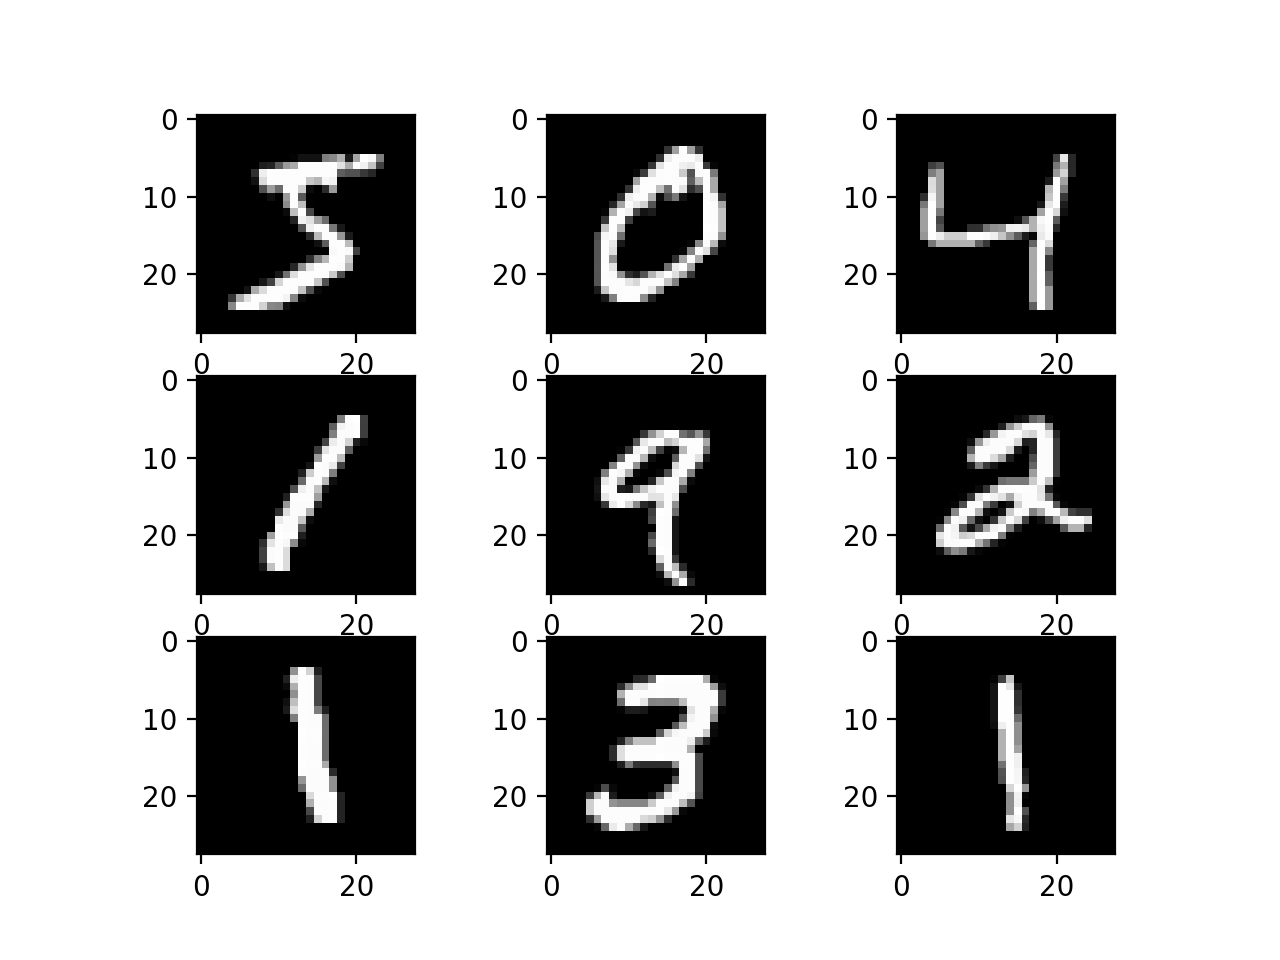
\includegraphics[width=0.8\textwidth]{mnist_example.png}
\end{center}


\end{document}
